\subsection{Ridge Regression}

Now we applied the Ridge Regression to perform selection. In figure \Fig~\ref{fig:RidgeCoefVsLambda} are shown the coefficients' behavior as $\lambda$ increases. 

\begin{figure}[h]
	\centering
	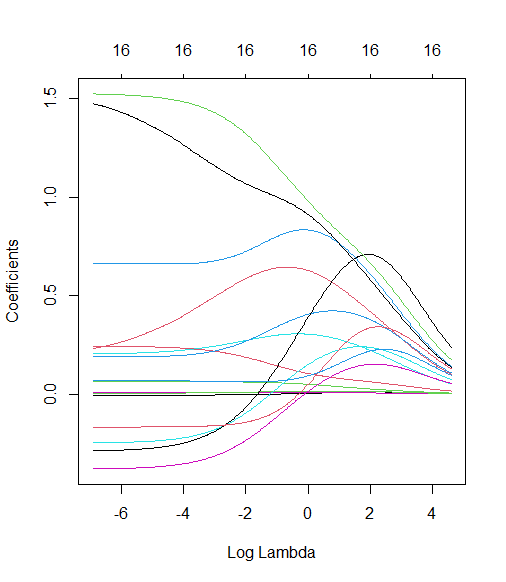
\includegraphics[width=0.4\linewidth]{ImageFiles/Regression/Ridge/RidgeCoefVsLambda}
	\caption{The ridge regression coefficients as function of $\lambda$.}
	\label{fig:RidgeCoefVsLambda}
\end{figure}

It's possible to observe that for $\lambda$ large enough, around $10^2$, all the coefficients tend become close to zero. However, they are never exactly zero.

To select the optimal value of the penalization factor $\lambda$ we employed "K-Fold Cross-Validation" with $K=10$. In figure \Fig~\ref{fig:RidgeCvPlot} is possible the trend of the cross validated MSE("\textit{Mean Square Error}") when $\lambda$ increases. The optimal value was found to be $\lambda_{opt} = 0.0304$.

\begin{figure}[h]
	\centering
	\begin{subfigure}{.6\textwidth}
		\centering
		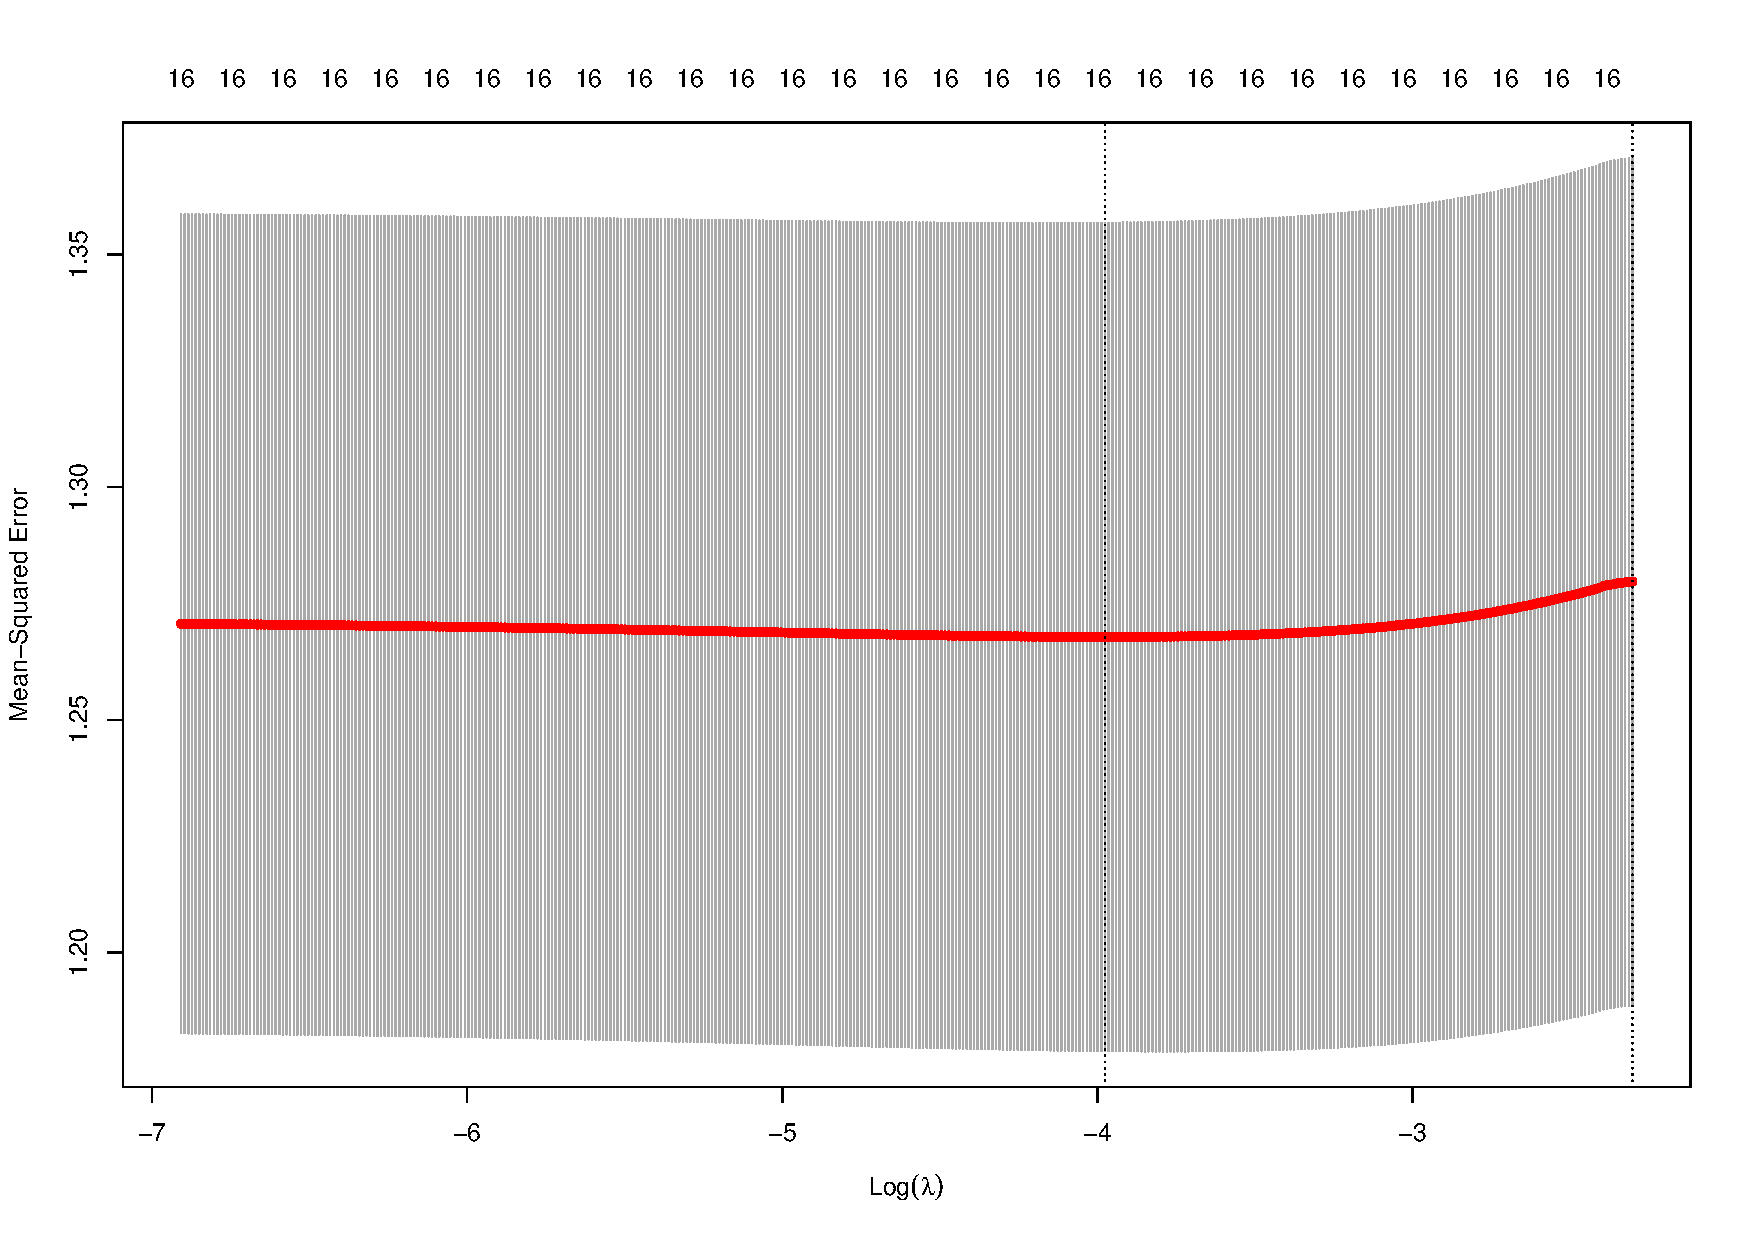
\includegraphics[width=0.7\linewidth]{ImageFiles/Regression/Ridge/RidgeCvPlot}
		\caption{The Cross Validated MSE as function of $\lambda$.}
		\label{fig:RidgeCvPlot}
	\end{subfigure}%
	\begin{subfigure}{.6\textwidth}
		\centering
		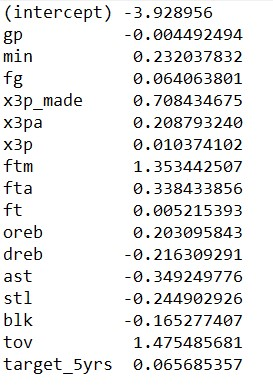
\includegraphics[width=0.4\linewidth]{ImageFiles/Regression/Ridge/FinalRidgeCoef}
		\caption{Ridge Regression coefficients with $\lambda_{opt}$.}
		\label{fig:FinalRidgeCoef}
	\end{subfigure}
\end{figure}

With optimal value of $\lambda$ obtained we fitted the final model and the coefficients are in figure \Fig~\ref{fig:FinalRidgeCoef}. For this model we computed also the test MSE and it is $MSE_{test} = 1.33$

In this case the Ridge Penalization does not reduce the number of coefficients, and it does not even improve significantly the MSE. We can then conclude that using Ridge Regression is not useful for our purposes.
